\subsubsection{Phase diagram}

\label{sec:phase-diagram}

In this phase diagram cookbook, phase diagrams are generated from model runs and visualized with VISIT. % intro
It is a simple way to check the implementation in material model with visible outputs.% motivation
The idea lies in initiating a linear temperature variation along the x-axis in a box geometry, so as to view the two axes as pressure and temperature, respectively. % technique
Here, I visualize a diagram of the phase transitions implemented in the ViscoPlastic material model, as well as a lookup table in the steinberg material model% examples

\paragraph{The input file.}
You can find the input file to run this cookbook example in \url{cookbooks/phase_diagram.prm}

\par The box extends 800 km * 800 km. % geometry
Initial temperature increases from 273 K on the left side to 2273 K on the right side. % initial conditions
Pressure, on the other hand, increases from the top of the box to the bottom with a constant gradient.
This is assured by assigning a constant density with zero expansivity.
It differs from a classic phase diagram only in the direction pressure increases.

\par Two compositions of pyrolite and harzburgite are included in the model. % composition
With each run, only one composition is assigned to the whole domain in order to visualize the diagrams of these two separately.

\par Material model is then set up to mimic mantle phase transitions at 410, 520, and 660 km.% setup of mantle transitions
Details of phase transitions are taken from \cite{billen2018decoupling}.
A trick of assigning the values of density to the field of thermal capacity is played here. % trick
This serves the goal of visualizing values of reference densities of phases with the 'real density' assigned with a constant value in the model.
Inputs for this material model is listed here:
\lstinputlisting[language=prmfile]{cookbooks/phase_diagram/doc/material_model.prm.out}


\paragraph{Results}

\par Visualization of model results yields a phase diagram of a pyrolitic mantle(Figure \ref{fig:phase_diagram_ph_density}). % phase diagram
The field shown here has the reference densities of the pyrolite phases, though settings of phase transitions are over-simplified.
One may notice that 3 transitions(i.e. one in the olivine system, two in the spinel system) are included for the 660 interfaces, % 3 transitons, higher T
and they need to be modified at a higher temperature.
In spite of the complexities of mantle phases, the focus of this first example is to simply illustrate this approach of visualizing it.
Beyond showing the diagram, I have also used the 'lineout' feature in VISIT to export the data along two vertical lines at T = 1173 and T = 1673 (Figure \ref{fig:phase_diagram_ph_profile}). % linear profile
The T = 1173 illustrates the buoyancy forces felt by a descending cold slab within the mantle transition zone.

\par Next, we shift to harzburgite by changing the values of the initial compositional field from 0 to 1.  % harzburgite
For this, what's needed is the following change:
\lstinputlisting[language=prmfile]{cookbooks/phase_diagram/doc/harzburgite.prm.out}
With that, we could also visualize the phase diagram of harzburgite in Figure \ref{fig:phase_diagram_ph_density}.

\par Moreover, I tested the a pyrolitic lookup table used in the Steiberg material model(Figure \ref{fig:phase_diagram_steinberg_density}).% steiberg model, todo fix reference
The same setup of the initial condition is applied as in the previous case. % initial condition
The densities, however, are not assigned to the heat capacity anymore.
Thus the vertical axis would deviate from the axis of pressure a little bit.
This serves the goal of illustrating a more complex and thus more realistic model of phase transitions.
Modification for the material model is listed below:
\lstinputlisting[language=prmfile]{cookbooks/phase_diagram/doc/steinberg.prm.out}  % todo add 


%%%%% figures %%%%%%
%%%%%%%%% figures1: pyrolite %%%%%%
\begin{figure}
\phantom.
\hfill
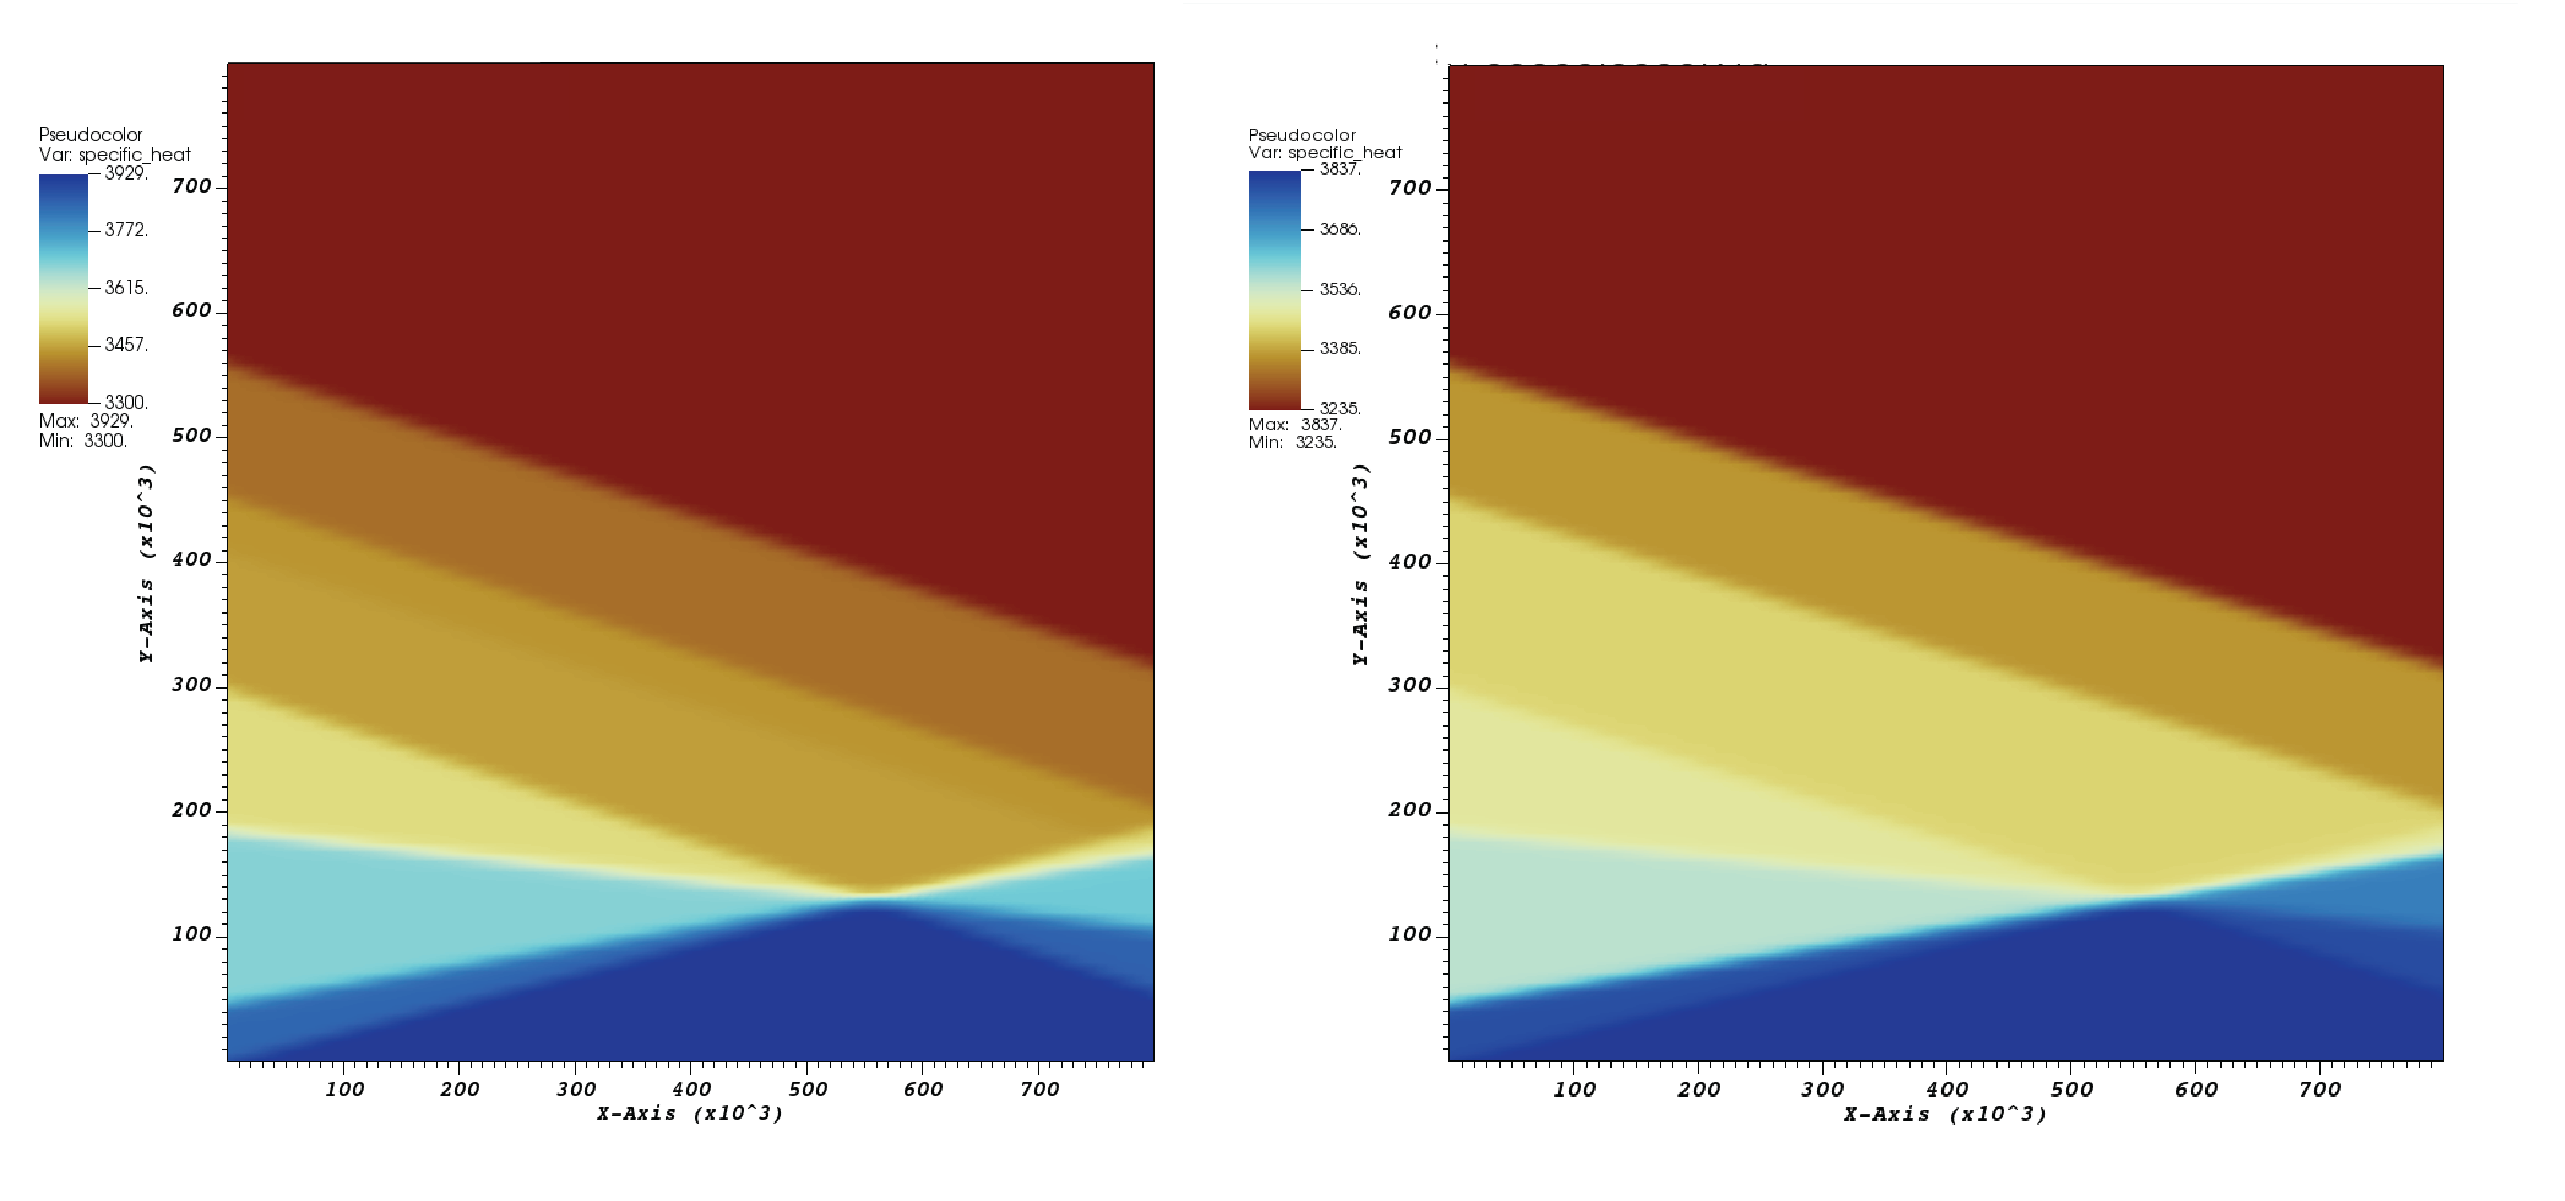
\includegraphics[width=0.9\textwidth]{cookbooks/phase_diagram/doc/pyrolite_harzburgite.png}
\hfill
\phantom.
\caption{\it The field of heat capacity showing values of reference densities for Pyrolitic and Harzburgitic phases.}
\label{fig:phase_diagram_ph_density}
\end{figure}

%%%%%%%%%% figures2: pyrolite profiles %%%%%%
\begin{figure}
\centering
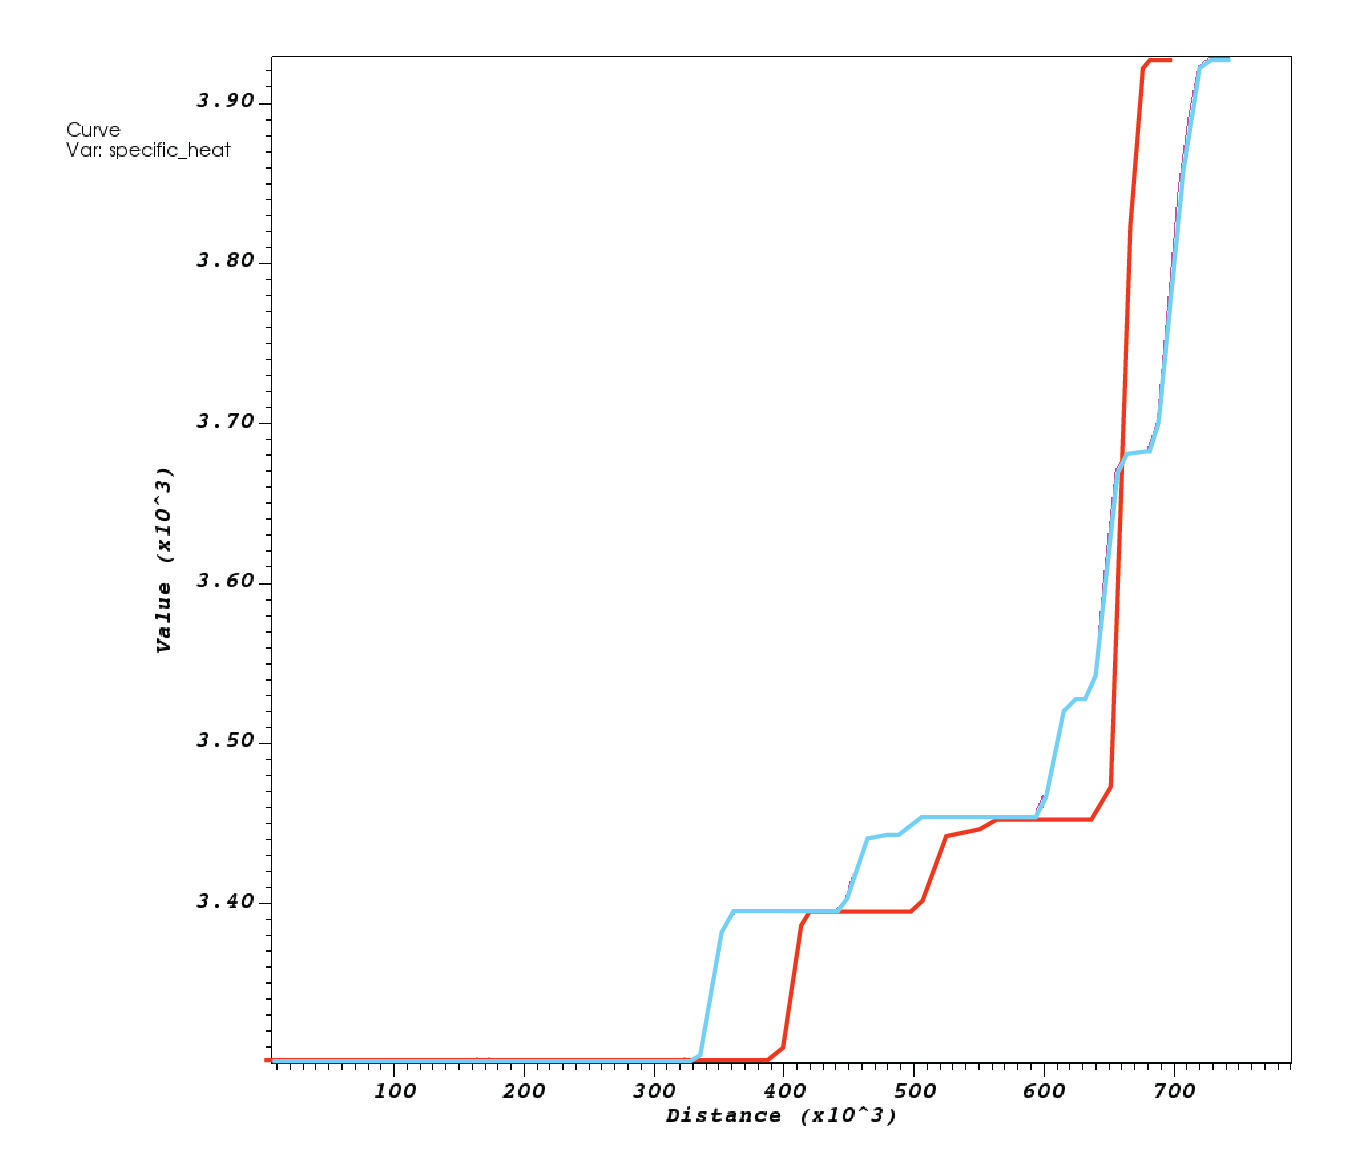
\includegraphics[width=0.4\textwidth]{cookbooks/phase_diagram/doc/pyrolite_linear.png}
\caption{\it Profiles of pyrolitic density at T=1173K(red) and 1673K(blue).}
\label{fig:phase_diagram_ph_profile}
\end{figure}
%%%%%%%%% figures3: lookup table %%%%%%
\begin{figure}
\centering
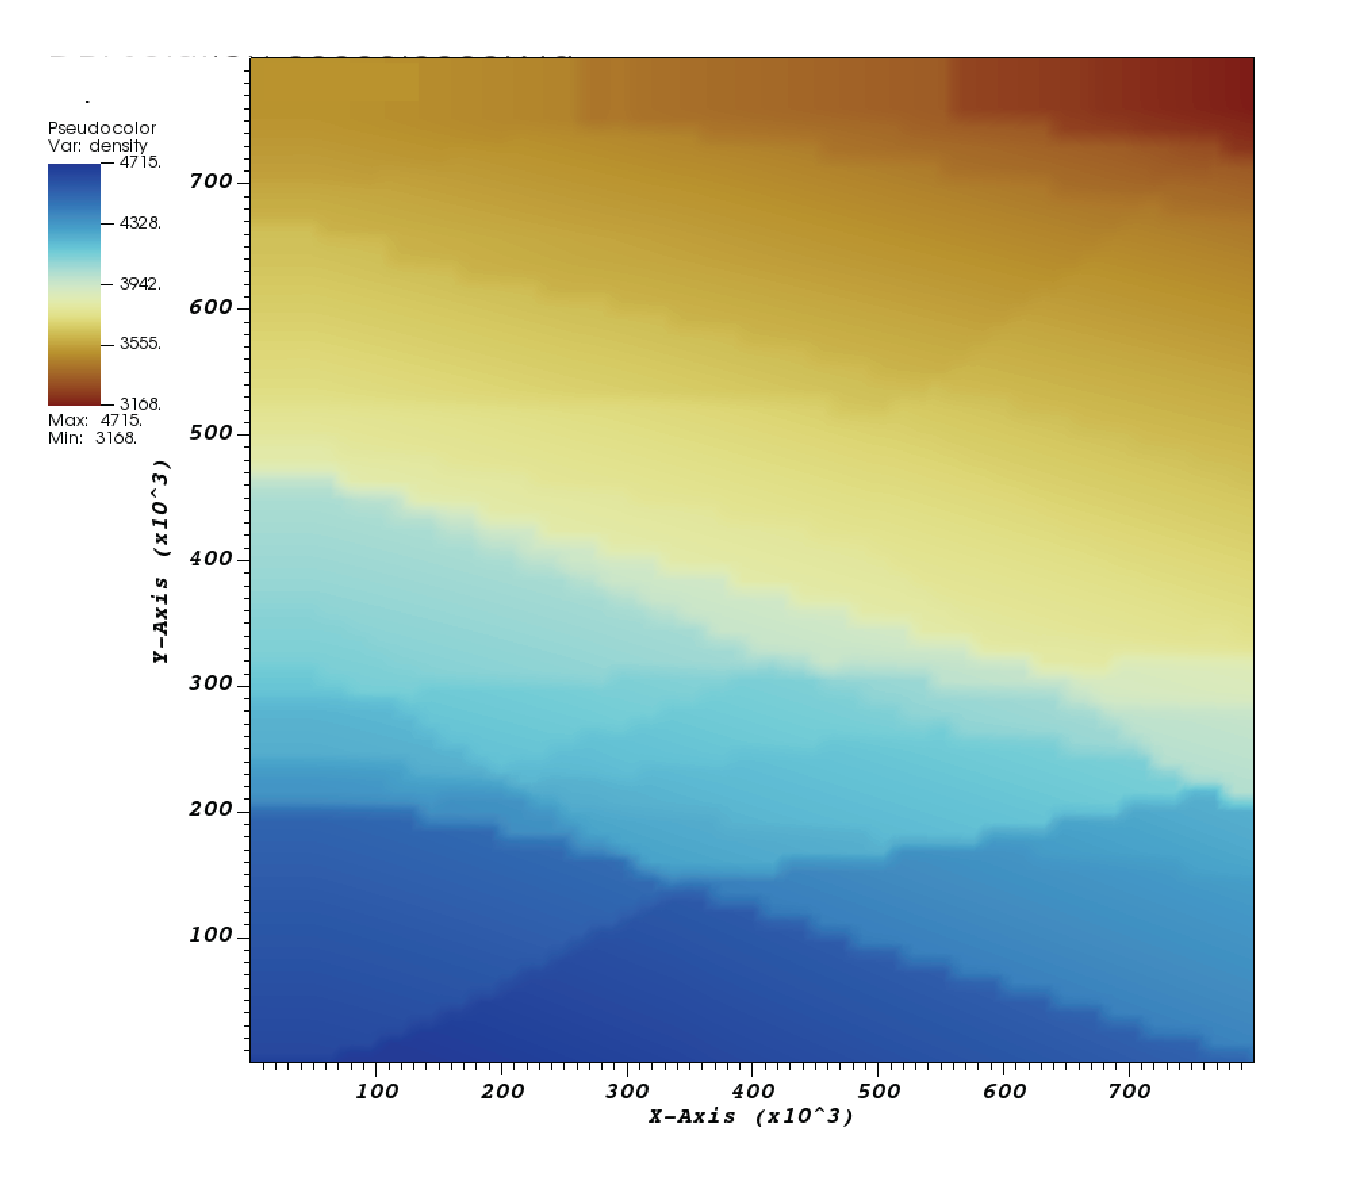
\includegraphics[width=0.4\textwidth]{cookbooks/phase_diagram/doc/steinberg.png}
\caption{\it Density from lookup table of pyrolite from \cite{stixrude2011thermodynamics}} % todo: cite
\label{fig:phase_diagram_steinberg_density}
\end{figure}
